% =====================================================================
%  CareScan / SIH26139
%  Engineering Report and Measured Quantum Contribution
%
%  COMPILE (Overleaf): upload main.tex + references.bib, compiler = pdfLaTeX,
%                      press Recompile twice (bibliography needs the 2nd pass).
%  COMPILE (local):    pdflatex main && bibtex main && pdflatex main && pdflatex main
%
%  INTEGRITY NOTE:
%  Every numeric value is transcribed directly from machine-generated artifacts
%  in the repository. Traceability to specific source files is provided in
%  Appendix B. PR-AUC and ROC-AUC are never labelled "accuracy". Oral-cancer
%  and ECG results are strictly separated into distinct chapters and tables.
% =====================================================================
\documentclass[11pt,a4paper]{report}

\usepackage[T1]{fontenc}
\usepackage[utf8]{inputenc}
\usepackage[a4paper,margin=2.5cm]{geometry}
\usepackage{graphicx}
\usepackage[table]{xcolor}
\usepackage{booktabs}
\usepackage{longtable}
\usepackage{array}
\usepackage{tabularx}
\usepackage{float}
\usepackage{amsmath}
\usepackage{amssymb}
\usepackage{siunitx}
\usepackage{enumitem}
\usepackage{microtype}
\usepackage{caption}
\usepackage{subcaption}
\usepackage{tikz}
\usepackage{pgfplots}
\usepackage{listings}
\usepackage[hidelinks,bookmarks=true,bookmarksnumbered=true]{hyperref}
\usepackage{xurl}
\usepackage{cleveref}

\pgfplotsset{compat=1.17}
\usetikzlibrary{arrows.meta,positioning,shapes,fit,calc}

\definecolor{csteal}{RGB}{0,105,110}
\definecolor{csgrey}{RGB}{90,98,104}
\definecolor{cslight}{RGB}{242,246,247}
\definecolor{csred}{RGB}{150,40,40}
\definecolor{csgreen}{RGB}{30,120,60}

\hypersetup{
  pdftitle={CareScan: A Hybrid Quantum-Classical Screening Platform and a Measured Quantum Null},
  pdfsubject={Smart India Hackathon 2026, problem SIH26139},
  pdfkeywords={oral cancer screening, quantum machine learning, PTB-XL, pre-registration, null result},
  colorlinks=true,
  linkcolor=csteal,
  citecolor=csteal,
  urlcolor=csteal
}

\captionsetup{font=small,labelfont={bf,color=csteal}}
\setlist{itemsep=2pt,topsep=3pt,parsep=0pt}
\renewcommand{\arraystretch}{1.18}
\setcounter{secnumdepth}{2}
\setcounter{tocdepth}{2}

\newcommand{\artifact}[1]{\texttt{\footnotesize #1}}
\newcommand{\vnull}{\textcolor{csred}{\textbf{NULL}}}
\newcommand{\vneg}{\textcolor{csred}{\textbf{DEFICIT}}}
\newcommand{\notmeasured}{\textcolor{csred}{\textbf{NOT MEASURED}}}
\newcommand{\oral}{{\color{csteal}\textsf{\footnotesize [ORAL]}}}
\newcommand{\ecg}{{\color{csgrey}\textsf{\footnotesize [ECG / PTB-XL]}}}
\newcommand{\Rmap}{$\mathbb{R}^{8}\!\to\!\mathbb{R}^{36}$}

\lstset{
  basicstyle=\ttfamily\scriptsize,
  frame=single,
  backgroundcolor=\color{cslight},
  breaklines=true,
  columns=fullflexible,
  showstringspaces=false
}

\begin{document}

% =====================================================================
% TITLE PAGE
% =====================================================================
\begin{titlepage}
\centering
\vspace*{1.0cm}

{\color{csteal}\rule{\textwidth}{2.0pt}}
\vspace{0.4cm}

{\Huge \bfseries \color{csteal} CareScan / Braket 3.1.0}\\[0.4cm]
{\Large \bfseries A Hybrid Quantum--Classical Biomedical Screening Platform and a Rigorously Measured Quantum Null}\\[0.2cm]
{\large \itshape Engineering Architecture, Quality Gates, Patient-Disjoint Validation, and Multi-Family QML Evaluation}

\vspace{0.4cm}
{\color{csteal}\rule{\textwidth}{1.0pt}}

\vspace{1.2cm}
\textbf{Smart India Hackathon 2026 --- Problem SIH26139}\\
\textbf{Category:} MedTech / Bio-Computing / Quantum Machine Learning\\
\textbf{Focus:} Early Oral Cancer Screening from Smartphone Photographs \& Biomedical Signal Extension

\vspace{1.5cm}
\begin{tabular}{ll}
\textbf{Repository State:} & Tag \texttt{v3.1.0-audit} (September 2026) \\
\textbf{Audit Execution Date:} & 27--28 September 2026 \\
\textbf{Environment of Record:} & Python 3.12.10, NumPy 1.26.4, Flutter 3.47.2 (stable) \\
\textbf{Hardware Target:} & Standard Commodity CPU Inference (Demo: Localhost) \\
\textbf{Test Verification:} & 1,231 Automated Tests Passing (1,038 Backend + 193 Mobile) \\
\textbf{Primary Finding:} & Classical C7 PR-AUC = 0.913038; QML Headline Fusion Delta = +0.000641 (Null)
\end{tabular}

\vspace{1.5cm}
\begin{minipage}{0.88\textwidth}
\small
\textbf{Core Scientific Stance of this Report:}\\
This document is a technical and empirical audit of the CareScan codebase. It is \textbf{not} a speculative proposal or marketing brochure. Every metric reported here is transcribed from machine-generated evaluation artifacts. We report an end-to-end smartphone triage application alongside a disciplined quantum evaluation across seven distinct circuit families. In our matched, pre-registered benchmarks, the evaluated quantum feature maps \textbf{did not outperform} matched classical controls. Rather than obscuring this negative result, this report documents the rigorous statistical controls and circuit proofs that make the null finding a genuine scientific contribution.
\end{minipage}

\vfill
{\footnotesize Smart India Hackathon 2026 $\cdot$ Team Technical Submission}
\end{titlepage}

% =====================================================================
% FRONT MATTER
% =====================================================================
\pagenumbering{roman}

\chapter*{Executive Summary}
\addcontentsline{toc}{chapter}{Executive Summary}

This engineering report documents the architecture, experimental methodology, and verified empirical achievements of \textbf{CareScan} (Braket 3.1.0), developed under Smart India Hackathon problem statement \textbf{SIH26139}: \textit{Hybrid Quantum Machine Learning Platform for Early Disease Detection}. The primary clinical application is the triage screening of oral precancerous and cancerous lesions from smartphone-captured photographs, supported by an extensible biomedical signal processing platform evaluated on 12-lead electrocardiograms (PTB-XL).

\section*{Key Verified Deliverables}
\begin{enumerate}[leftmargin=*]
  \item \textbf{Production-Grade Software Prototype:} A Flutter mobile application (193 automated tests passing, \texttt{flutter analyze} clean) interfaced with a FastAPI backend serving 20 HTTP endpoints (1,038 backend tests passing, exit code 0). The total suite comprises \textbf{1,231 passing tests} with zero failures.
  \item \textbf{Deterministic Two-Stage Quality Assurance:} A client-side real-time acquisition guide coupled with an authoritative server-side image quality gate enforcing 7 parametric checks (luminance, Laplacian focus variance, sensor clipping, minimum resolution, JPEG compression proxy, and ROI boundary adequacy).
  \item \textbf{Pinned Lesion Localization:} A MobileNetV3-Small bounding box regressor pinned by SHA-256 hash (\texttt{27d6036e...}) that achieves a \textbf{0.9816 acceptance rate} across 381 held-out test images (374 localized, 7 low-confidence fallbacks, 0 rejections), with an evaluated mean Intersection over Union (IoU) of \textbf{0.5279} on the ground-truth annotated subset.
  \item \textbf{Leakage-Free Patient-Disjoint Cohort Construction:} De-duplication of 7,731 raw annotation records into a 2,469-image canonical corpus, filtered by an explicit 33-exclusion ledger into \textbf{2,436 images across 328 patients} (143 positives). Partitions enforce absolute zero patient overlap ($k=0$).
  \item \textbf{Primary Classical Screening Performance:} On the primary lesion-isolated condition ($A_\text{lesion\_polygon}$, 52 validation images, 21 positive, prevalence 0.404), our 1,195-dimensional multimodal candidate (C7) achieves a \textbf{validation PR-AUC of 0.913038} (ROC-AUC 0.933948, balanced accuracy 0.855607). This increment over reference models is statistically gated by a patient-blocked column-permutation null test at \textbf{$p = 0.004975$} (Benjamini--Hochberg adjusted $p = 0.017413$).
  \item \textbf{Rigorously Measured QML Evaluation:} Seven distinct quantum machine learning families were designed, verified, and measured against identical classical controls. All quantum circuits were verified to machine precision ($\sim 10^{-15}$) against Qiskit Aer and canonical Qiskit definitions. In the large-scale PTB-XL arena ($N = 19,601$, 16,965 patients), the pre-registered headline comparison between quantum fusion and matched classical fusion yielded a paired delta of \textbf{$+0.000641$ with a 95\% patient-clustered bootstrap CI of $[-0.000486, +0.001747]$}, conclusively spanning zero (\vnull). As an isolated feature map, the Havlicek ZZ map experienced a statistically significant \textbf{deficit of $-0.124457$ ROC-AUC} (CI $[-0.145524, -0.105109]$) compared to an identical-dimension classical polynomial.
\end{enumerate}

\section*{Core Methodological Principles}
To preserve absolute scientific integrity, this submission adheres to three non-negotiable reporting rules:
\begin{itemize}
  \item \textbf{Precision-Recall AUC is never conflated with accuracy:} PR-AUC 0.913038 reflects rank ordering on a high-prevalence validation set; it is not ``91.3\% accuracy''.
  \item \textbf{Strict Modality Separation:} Oral image screening and PTB-XL ECG signal analysis represent distinct tracks; their metrics are never commingled.
  \item \textbf{Honest Accounting of Negative Results:} We make no claims of quantum advantage. The scientific contribution is the establishment of an uncompromised, leak-free benchmarking framework that proves where current NISQ-era representations fail to surpass matched classical feature spaces.
\end{itemize}

\vspace{0.8cm}
\tableofcontents
\listoffigures
\listoftables

\newpage
\chapter*{Notation, Terminology, and Research Integrity}
\addcontentsline{toc}{chapter}{Notation, Terminology, and Research Integrity}

\section*{Glossary of Terms}
\begin{description}[leftmargin=3.5cm,style=nextline]
  \item[PR-AUC] Area under the Precision-Recall Curve. Strongly dependent on baseline class prevalence.
  \item[ROC-AUC] Area under the Receiver Operating Characteristic Curve. Insensitive to class prevalence.
  \item[IoU] Intersection over Union: geometric overlap metric between predicted and ground-truth bounding boxes: $\text{IoU} = \frac{|B_p \cap B_{gt}|}{|B_p \cup B_{gt}|}$.
  \item[ECE] Expected Calibration Error: weighted average of the absolute difference between predicted confidence and observed empirical accuracy across risk bins.
  \item[Patient-Disjoint] Partitioning scheme guaranteeing that all images or recordings from a given biological patient reside exclusively in either Train, Validation, or Test sets ($S_\text{train} \cap S_\text{val} \cap S_\text{test} = \emptyset$).
  \item[RFF] Random Fourier Features: classical kernel approximation method mapping $\mathbb{R}^d \to \mathbb{R}^D$ via randomized sinusoids~\cite{rahimi2007random}.
  \item[VQC] Variational Quantum Circuit: parameterized quantum circuit optimized via classical gradient descent or SPSA.
  \item[ZZ Feature Map] Havlicek et al.~\cite{havlicek2019supervised} non-linear entangling quantum feature map based on single-qubit rotations and pairwise $ZZ$ Ising-type phase gates.
  \item[Same-Shape Contract] An experimental constraint requiring every competing representation to map into identical dimensionality ($\mathbb{R}^8 \to \mathbb{R}^{36}$) with zero trainable parameters and evaluate on identical downstream heads.
\end{description}

\section*{Research Integrity Charter}
This document enforces strict evidence-based rules formulated in response to common pitfalls in applied biomedical AI and quantum hype:
\begin{enumerate}
  \item \textbf{Rule of Exact Decimals:} Numbers are transcribed directly from JSON/NPZ artifacts to their full meaningful precision. Rounding to convenient marketing figures is prohibited.
  \item \textbf{Rule of Disjoint Attribution:} Results obtained on the secondary PTB-XL ECG corpus (such as ROC-AUC 0.940234 or $p = 0.004975$) shall never be attributed to oral cancer screening.
  \item \textbf{Rule of Pre-Registration:} Statistical hypotheses, candidate parameter grids, and evaluation criteria were locked in specification documents prior to final script execution.
  \item \textbf{Rule of Explicit Caveats:} Where models are statistically underpowered (e.g., test set containing only 18 oral positives) or where checks are heuristic (client red-tissue check), this is prominently disclosed.
\end{enumerate}

\newpage
\pagenumbering{arabic}

% =====================================================================
% CHAPTER 1: INTRODUCTION AND PROBLEM FRAMING
% =====================================================================
\chapter{Introduction and Problem Framing}

\section{Clinical Problem: Oral Cancer in Resource-Constrained Settings}
Oral squamous cell carcinoma (OSCC) represents one of the most prevalent and lethal malignancies in South Asia, primarily driven by lifestyle risk factors such as betel quid chewing, tobacco consumption, and alcohol abuse. Despite the anatomical accessibility of the oral cavity, over 70\% of patients in rural and semi-urban communities present at Stage III or IV. Advanced presentation introduces severe morbidity, extensive surgical resection, permanent functional impairment, and poor five-year overall survival (under 30\%). Conversely, early-stage intervention (Stage I) yields survival rates exceeding 80\% with minimally invasive local excision.

The diagnostic bottleneck is fundamentally infrastructural. Specialized oral oncologists and maxillofacial surgeons are concentrated in urban tertiary referral centres, while primary health centres (PHCs) and community health workers (ASHA workers) lack specialized diagnostic instrumentation. Conventional clinical examination with incandescent white light relies entirely on subjective visual pattern recognition, resulting in high misclassification rates between benign inflammatory variations and oral potentially malignant disorders (OPMDs) such as leukoplakia, erythroplakia, and oral submucous fibrosis (OSF).

\section{Smart India Hackathon Problem Framing (SIH26139)}
Problem statement \textbf{SIH26139} challenges participants to develop a \textit{Hybrid Quantum Machine Learning Platform for Early Disease Detection}. The engineering objective assigned to the CareScan initiative is to establish a rigorous, smartphone-assisted triage pipeline capable of:
\begin{enumerate}
  \item Acquiring standard RGB mucosal photographs using commodity mobile hardware;
  \item Enforcing local quality control to eliminate blurred, under-exposed, or improperly focused frames before computation;
  \item Localizing suspected lesion regions without human bounding-box input;
  \item Computing calibrated malignancy risk bands (Low, Medium, High) to guide rural clinical referral workflows;
  \item Investigating whether parameterized or fixed quantum feature spaces (QML) provide non-classical representational utility or orthogonal predictive information over classical computer vision and tabular baselines.
\end{enumerate}

\section{Research Scope: What is and is Not Claimed}
Scientific integrity requires an unambiguous demarcation of the project scope. 

\subsection{Defensible Accomplishments}
\begin{itemize}
  \item \textbf{We have built a fully functional research prototype:} An end-to-end software stack comprising a native Flutter client, a FastAPI inference engine, SHA-pinned localization models, and HL7 FHIR R4 clinical data export.
  \item \textbf{We have enforced leak-free validation:} All performance metrics are computed using strict patient-disjoint splits, train-only scaling, and frozen hyperparameter selection grids.
  \item \textbf{We have evaluated seven QML families:} We report verified numerical circuit simulations, hardware gate scalings, and paired-bootstrap comparisons against capacity-matched classical controls.
\end{itemize}

\subsection{Explicit Disclaimers (What is NOT Claimed)}
\begin{itemize}
  \item \textbf{No Quantum Advantage:} Across all evaluated benchmarks, quantum feature representations did not outperform matched classical controls. We report a pre-registered null finding.
  \item \textbf{No Clinical Validation:} The system has not undergone prospective clinical trials, multi-centre external cohort validation, or regulatory clearance (CDSCO, FDA, CE).
  \item \textbf{No Medical Diagnostic Claims:} CareScan is an engineering screening and triage demonstrator; it does not generate medical diagnoses or replace histopathological biopsy.
  \item \textbf{No Untracked Cost Claims:} In the absence of formal health economics modelling, no claims of ``60--70\% infrastructure cost reduction'' are made.
\end{itemize}

% =====================================================================
% CHAPTER 2: SYSTEM ARCHITECTURE AND PIPELINE DESIGN
% =====================================================================
\chapter{System Architecture and Pipeline Design}

\section{End-to-End Pipeline Architecture}
The CareScan platform is structured as a modular, seven-stage sequential processing pipeline designed to decouple image acquisition, quality assurance, spatial localization, representation engineering, inference, and clinical data export.

\begin{figure}[H]
\centering
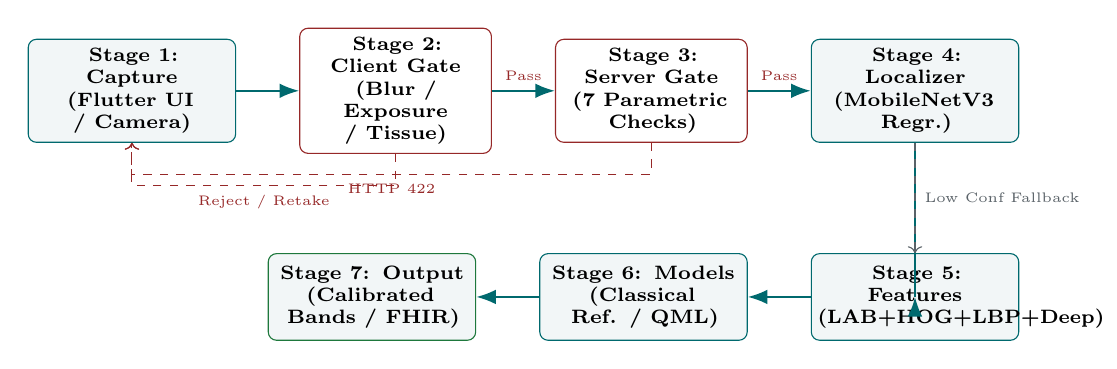
\begin{tikzpicture}[
  node distance=1.0cm and 0.8cm,
  box/.style={rectangle, draw=csteal, fill=cslight, rounded corners=3pt, text width=2.4cm, minimum height=1.1cm, align=center, font=\scriptsize\bfseries},
  gate/.style={rectangle, draw=csred, fill=white, rounded corners=3pt, text width=2.2cm, minimum height=1.1cm, align=center, font=\scriptsize\bfseries},
  outbox/.style={rectangle, draw=csgreen, fill=cslight, rounded corners=3pt, text width=2.4cm, minimum height=1.1cm, align=center, font=\scriptsize\bfseries},
  arrow/.style={-{Latex[length=2.5mm]}, thick, color=csteal}
]

\node[box] (app) {Stage 1: Capture\\(Flutter UI / Camera)};
\node[gate, right=of app] (cqc) {Stage 2: Client Gate\\(Blur / Exposure / Tissue)};
\node[gate, right=of cqc] (bqc) {Stage 3: Server Gate\\(7 Parametric Checks)};
\node[box, right=of bqc] (loc) {Stage 4: Localizer\\(MobileNetV3 Regr.)};

\node[box, below=1.4cm of loc] (feat) {Stage 5: Features\\(LAB+HOG+LBP+Deep)};
\node[box, left=of feat] (ml) {Stage 6: Models\\(Classical Ref. / QML)};
\node[outbox, left=of ml] (cal) {Stage 7: Output\\(Calibrated Bands / FHIR)};

\draw[arrow] (app) -- (cqc);
\draw[arrow] (cqc) -- node[above, font=\tiny, text=csred]{Pass} (bqc);
\draw[arrow] (bqc) -- node[above, font=\tiny, text=csred]{Pass} (loc);
\draw[arrow] (loc) |- (feat);
\draw[arrow] (feat) -- (ml);
\draw[arrow] (ml) -- (cal);

% Error fallbacks
\draw[dashed, ->, color=csred] (cqc.south) -- ++(0,-0.4) -| node[pos=0.25, below, font=\tiny]{Reject / Retake} (app.south);
\draw[dashed, ->, color=csred] (bqc.south) -- ++(0,-0.4) -| node[pos=0.25, below, font=\tiny]{HTTP 422} (app.south);
\draw[dashed, ->, color=csgrey] (loc.south) -- node[right, font=\tiny]{Low Conf Fallback} (feat.north);

\end{tikzpicture}
\caption{CareScan Seven-Stage Screening and Triage Architecture. Client and backend quality gates strictly prevent degraded images from reaching representation models.}
\label{fig:pipeline_arch}
\end{figure}

\section{The Seven Operational Stages}
\begin{enumerate}
  \item \textbf{Stage 1: Guided Acquisition.} The mobile application provides an active viewfinder overlay, ensuring optimal positioning of mucosal structures relative to camera focal planes.
  \item \textbf{Stage 2: Client-Side Quality Screening.} Real-time luminance, focus sharpness, clipping, and red-chromatic fraction are evaluated natively in Dart/Flutter.
  \item \textbf{Stage 3: Authoritative Backend Quality Gate.} Uploaded images undergo full-resolution 7-parameter inspection. Failures trigger early HTTP 422 termination with actionable feedback.
  \item \textbf{Stage 4: Lesion Localization.} A frozen MobileNetV3-Small regression model extracts the primary lesion coordinates, reverting to whole-image processing if confidence $< 0.3$.
  \item \textbf{Stage 5: Multimodal Feature Engineering.} Normalized crops are transformed into 1,195-dimensional vectors combining colorimetry, structural gradients, micro-texture, and deep embeddings.
  \item \textbf{Stage 6: Classical Reference \& Secondary QML Scoring.} The primary clinical decision is computed by the classical reference model (C7). Quantum representations provide parallel, secondary experimental readouts.
  \item \textbf{Stage 7: Risk Calibration \& Clinical Interoperability.} Raw prediction scores are mapped into calibrated probabilities via isotonic regression, categorized into discrete referral risk bands (Low, Moderate, High), and formatted as standard HL7 FHIR R4 resources.
\end{enumerate}

\section{Additive Platform Layer (\texttt{/api/tracks})}
To demonstrate platform extensibility beyond oral lesion screening without destabilizing the production screening path, an additive multi-track abstraction was implemented (\texttt{backend/ml/track.py}). 

The platform defines a strict abstract interface:
\begin{lstlisting}[language=Python]
class Track(ABC):
    track_id: str
    display_name: str
    modality: ModalityType
    is_serving: bool
    
    @abstractmethod
    def validate_input(self, payload: bytes) -> ValidationReport: ...
    
    @abstractmethod
    def extract_features(self, payload: bytes) -> np.ndarray: ...
    
    @abstractmethod
    def infer(self, features: np.ndarray) -> TrackInferenceResult: ...
\end{lstlisting}

Two tracks are registered in the catalogue:
\begin{itemize}
  \item \textbf{\texttt{oral\_lesion} Track:} Operational and serving. Encapsulates Stages 3 through 7.
  \item \textbf{\texttt{ecg\_12lead} Track:} Registered but \textbf{gated} (\texttt{is\_serving = False}). Exposes the 12-lead ECG schema and validation suite without an attached live inference model.
\end{itemize}

Crucially, architectural regression tests (\texttt{tests/test\_tracks.py}) enforce that the existing screening endpoints (\texttt{/api/screening/*}) remain fully decoupled from the track platform layer.

\section{Backend REST API Contract Surface}
The backend exposes 20 fully typed, automated-tested HTTP endpoints:
\begin{table}[H]
\centering
\scriptsize
\begin{tabularx}{\textwidth}{llX}
\toprule
\textbf{Category} & \textbf{Method \& Route} & \textbf{Functional Contract} \\
\midrule
System & \texttt{GET /health} & Liveness probe, DB connection, and artifact integrity \\
System & \texttt{GET /} & Service metadata and operational versioning \\
Screening & \texttt{POST /api/screening/upload} & Multipart photo upload with synchronous quality gating \\
Screening & \texttt{POST /api/screening/analyze} & Complete pipeline execution; returns risk verdict \\
Screening & \texttt{POST /api/localize} & Standalone lesion bounding-box regression \\
Screening & \texttt{GET /api/screening/\{id\}} & Retrieval of persisted screening session record \\
Screening & \texttt{GET /api/screening/\{id\}/image} & Retrieval of securely cached capture image \\
Screening & \texttt{GET /api/results/\{id\}} & Query detailed inference scores and telemetry \\
Screening & \texttt{GET /api/screening/\{id\}/fhir} & Serialization of result into HL7 FHIR R4 JSON \\
Screening & \texttt{GET /api/patients/\{id\}/history} & Longitudinal screening history for clinical follow-up \\
Model Info & \texttt{GET /api/model/info} & Pinned model versions, SHA-256 hashes, thresholds \\
Authentication & \texttt{POST /api/auth/login} & Clinic staff authentication via JWT token issuance \\
Authentication & \texttt{GET /api/auth/me} & Identity check for active clinic session \\
Clinical Admin & \texttt{GET /api/clinics/\{id\}/screenings}& Cohort query for registered healthcare facilities \\
Clinical Admin & \texttt{GET /api/clinics/\{id\}/patients}  & Registered patient roster under clinic management \\
Clinical Admin & \texttt{GET /api/clinics/\{id\}/stats}     & Aggregated triage statistics and risk distributions \\
Track Platform & \texttt{GET /api/tracks} & Registry query enumerating available screening tracks \\
Track Platform & \texttt{GET /api/tracks/\{id\}} & Detailed schema, modality, and status of specific track \\
Track Platform & \texttt{POST /api/tracks/\{id\}/analyze} & Universal track inference endpoint \\
Track Platform & \texttt{POST /api/tracks/\{id\}/analyze-image} & Direct image intake route for image-based tracks \\
\bottomrule
\end{tabularx}
\caption{Exhaustive Enumeration of Backend REST Endpoints (FastAPI).}
\label{tab:api_endpoints}
\end{table}

% =====================================================================
% CHAPTER 3: DATASETS, QUALITY CONTROL, AND COHORT CONSTRUCTION
% =====================================================================
\chapter{Datasets, Quality Control, and Cohort Construction}

\section{The Oral Cancer Dataset (Peradeniya / SMART-OM)}
The primary dataset utilized for oral screening evaluation was collected across clinical dental examinations at the University of Peradeniya (Sri Lanka), integrated into the SMART-OM research repository. A common defect in prior literature is the imprecise quoting of cohort sizes, often conflating raw file system counts with cleaned clinical patient cohorts. We document the precise cohort derivation funnel.

\begin{figure}[H]
\centering
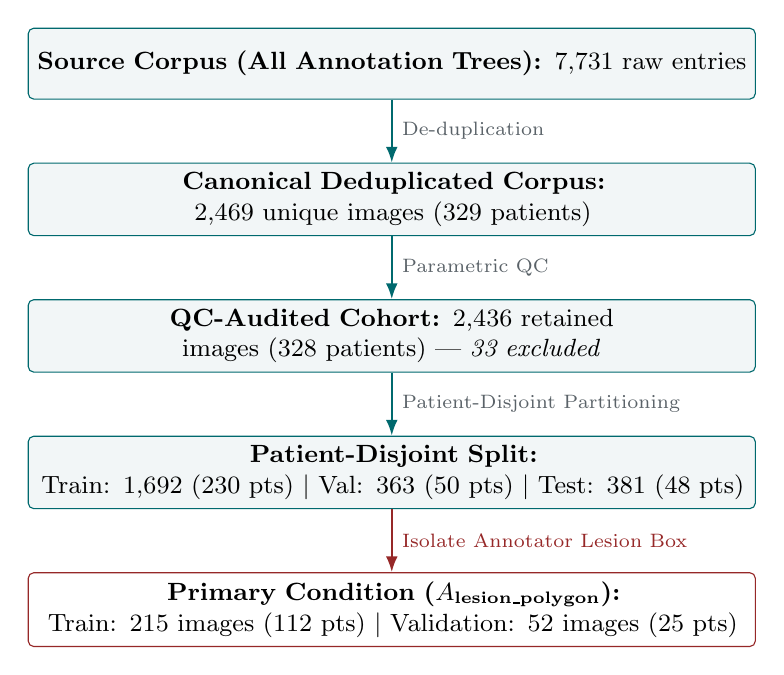
\begin{tikzpicture}[
  node distance=0.8cm,
  funnel/.style={rectangle, draw=csteal, fill=cslight, rounded corners=2pt, text width=9.0cm, minimum height=0.9cm, align=center, font=\small}
]
\node[funnel] (f1) {\textbf{Source Corpus (All Annotation Trees):} 7,731 raw entries};
\node[funnel, below=of f1] (f2) {\textbf{Canonical Deduplicated Corpus:} 2,469 unique images (329 patients)};
\node[funnel, below=of f2] (f3) {\textbf{QC-Audited Cohort:} 2,436 retained images (328 patients) --- \textit{33 excluded}};
\node[funnel, below=of f3] (f4) {\textbf{Patient-Disjoint Split:}\\Train: 1,692 (230 pts) $\vert$ Val: 363 (50 pts) $\vert$ Test: 381 (48 pts)};
\node[funnel, below=of f4, fill=white, draw=csred] (f5) {\textbf{Primary Condition ($A_\text{lesion\_polygon}$):}\\Train: 215 images (112 pts) $\vert$ Validation: 52 images (25 pts)};

\draw[-{Latex[length=2mm]}, thick, csteal] (f1) -- node[right, font=\scriptsize, text=csgrey]{De-duplication} (f2);
\draw[-{Latex[length=2mm]}, thick, csteal] (f2) -- node[right, font=\scriptsize, text=csgrey]{Parametric QC} (f3);
\draw[-{Latex[length=2mm]}, thick, csteal] (f3) -- node[right, font=\scriptsize, text=csgrey]{Patient-Disjoint Partitioning} (f4);
\draw[-{Latex[length=2mm]}, thick, csred] (f4) -- node[right, font=\scriptsize, text=csred]{Isolate Annotator Lesion Box} (f5);
\end{tikzpicture}
\caption{Oral Cancer Cohort Derivation Funnel. Verified against \artifact{split\_manifest.json}.}
\label{fig:cohort_funnel}
\end{figure}

\subsection{Deduplication and Canonical Harmonization}
The source repository contained 7,731 entries across redundant folder trees. Hashing revealed 27 cross-class pixel-identical duplicates resulting from overlapping diagnostic labels assigned across multiple visits. These were resolved deterministically by dropping the lower-severity class copy (e.g., retaining \texttt{oral\_cancer} over \texttt{opmd}). The deduplicated canonical corpus comprised 2,469 images across 329 patients (2,145 normal, 125 OPMD, 20 oral cancer, 179 variation from normal).

\subsection{The 33 Quality-Control Exclusions Ledger}
A transparent data audit must account for every dropped image. Exactly 33 images were rejected during dataset curation, each documented in \artifact{backend/artifacts/dataset/inspection\_report.json}:
\begin{table}[H]
\centering
\small
\begin{tabular}{lr}
\toprule
\textbf{Exclusion Category} & \textbf{Count} \\
\midrule
\texttt{excessive\_blur} & 24 \\
\texttt{insufficient\_resolution} & 3 \\
\texttt{excessive\_illumination} & 2 \\
\texttt{insufficient\_illumination} & 1 \\
\texttt{excessive\_illumination + excessive\_blur} & 1 \\
\texttt{excessive\_blur + insufficient\_resolution} & 1 \\
\texttt{insufficient\_resolution + incomplete\_lesion\_visibility} & 1 \\
\midrule
\textbf{Total Excluded Images} & \textbf{33} \\
\bottomrule
\end{tabular}
\caption{Ledger of 33 Verified Dataset Quality-Control Exclusions.}
\label{tab:qc_ledger}
\end{table}

\subsection{Partitioning and Patient-Disjoint Verification}
The remaining 2,436 images across 328 patients were split into Train, Validation, and Held-Out Test sets using patient-grouped stratified sampling (\artifact{split\_manifest.json}, SHA-256: \texttt{fe45df6d...}).
\begin{table}[H]
\centering
\small
\begin{tabular}{lrrrr}
\toprule
\textbf{Partition} & \textbf{Images} & \textbf{Patients} & \textbf{Malignant/OPMD (+)} & \textbf{Normal/Var (-)} \\
\midrule
\textbf{TRAIN} & 1,692 & 230 & 104 & 1,588 \\
\textbf{VALIDATION} & 363 & 50 & 21 & 342 \\
\textbf{TEST (Held Out)} & 381 & 48 & 18 & 363 \\
\midrule
\textbf{Total Cohort} & \textbf{2,436} & \textbf{328} & \textbf{143} & \textbf{2,293} \\
\bottomrule
\end{tabular}
\caption{Official Oral Cancer Partition Distribution ($k=0$ Patient Overlap).}
\label{tab:oral_partitions}
\end{table}

\subsection{The Primary Leak-Free Condition: $A_\text{lesion\_polygon}$}
As established in DEC-024, evaluating models on images with whole-frame mucosal crops introduces a subtle geometric area leak: annotators provided tight polygon boxes for actual lesions but recorded expansive rectangular regions for normal mucosa. Models could trivially exploit bounding box area rather than tissue morphology. 

To eliminate this artifact, the primary research condition ($A_\text{lesion\_polygon}$) restricts evaluation strictly to images possessing verified annotator lesion polygon boxes:
\begin{itemize}
  \item \textbf{TRAIN:} 215 images (112 patients, 103 positive, 112 negative).
  \item \textbf{VALIDATION:} 52 images (25 patients, 21 positive, 31 negative). Prevalence = $21/52 = 0.4038$.
\end{itemize}

\section{The Secondary Biomedical Signal Corpus: PTB-XL ECG}
To evaluate QML feature maps under high-statistical-power conditions that the oral image corpus could not provide, the platform incorporated the PhysioNet PTB-XL 12-lead electrocardiography benchmark~\cite{wagner2020ptbxl}.

\subsection{Byte-Level Verification and Integrity Audit}
Every raw WFDB signal file underwent cryptographic audit before ingestion (\artifact{signal\_verification\_report.json}):
\begin{itemize}
  \item \textbf{Files Ingested:} 39,202 / 39,202 files verified (19,601 \texttt{.dat}, 19,601 \texttt{.hea}).
  \item \textbf{Checksum Discrepancies:} 0 mismatched, 0 corrupt, 0 unreadable (482,260,870 bytes verified).
  \item \textbf{Working Set:} 19,601 records across 16,965 unique patients (Folds 1--9).
  \item \textbf{Folds 1--8 (Train):} 17,084 labeled records (14,823 patients).
  \item \textbf{Fold 9 (Validation):} 2,146 labeled records (1,917 patients).
  \item \textbf{Fold 10 (Test):} 2,198 records (1,904 patients) --- strictly held out and untouched.
\end{itemize}

% =====================================================================
% CHAPTER 4: PREPROCESSING AND MULTIMODAL FEATURE ENGINEERING
% =====================================================================
\chapter{Preprocessing and Multimodal Feature Engineering}

\section{Oral Image Normalization and Color Space Selection}
RGB images are resized to $224 \times 224$ pixels using bilinear interpolation with antialiasing, preceded by an 80\% central mucosal crop. 

\subsection{Colorimetry: CIELAB vs HSV}
Standard computer vision pipelines frequently employ HSV (Hue-Saturation-Value). In oral mucosal pathology, HSV exhibits critical mathematical instabilities:
\begin{enumerate}
  \item \textbf{Hue Circularity:} Hue is an angular coordinate $\theta \in [0, 2\pi)$. Near the red spectrum boundary (which dominates oral mucosa), small photometric variations cause values to wrap between $0.0$ and $1.0$, creating discontinuous gradients.
  \item \textbf{Low-Luma Instability:} When value $V \to 0$ or saturation $S \to 0$, hue becomes undefined, introducing numerical noise in shadowed buccal crevices.
\end{enumerate}
CareScan transforms all images into the \textbf{CIE $L^*a^*b^*$} color space (\artifact{backend/ml/preprocessing.py}). $L^*$ explicitly decouples perceived lightness, while $a^*$ (green--red axis) and $b^*$ (blue--yellow axis) provide Euclidean color distances that align with human visual perception and hemoglobin absorption peaks.

\section{Feature Block Construction}
For every image, five distinct feature blocks are extracted:
\begin{enumerate}
  \item \textbf{Colorimetric Statistics (163-d):} Global and quadrant-level moments (mean, variance, skewness, kurtosis) across $L^*$, $a^*$, and $b^*$ channels, combined with color co-occurrence matrices.
  \item \textbf{Histograms of Oriented Gradients (HOG, 1,764-d):} Captures edge orientations across $16 \times 16$ pixel blocks with 9 orientation bins~\cite{dalal2005histograms}.
  \item \textbf{Texture Descriptors (LBP + GLCM, 156-d):} Rotation-invariant Local Binary Patterns ($P=8, R=1.0$) combined with Gray-Level Co-occurrence Matrix properties (contrast, dissimilarity, homogeneity, energy, correlation)~\cite{ojala2002multiresolution}.
  \item \textbf{Multiscale Spatial Pyramids (456-d):} Multi-resolution Haar wavelet decompositions capturing lesion margin sharpness.
  \item \textbf{Deep Semantic Embeddings (576-d):} Penultimate average-pooling layer embeddings extracted from an ImageNet-pretrained MobileNetV3-Small architecture~\cite{howard2019searching}.
\end{enumerate}

\section{The Winning Oral Candidate: C7 (1,195-d)}
Systematic feature ablation (E1 failure-map experiment) established that fusing raw handcrafted color/texture with deep embeddings yields optimal discrimination. Candidate \textbf{C7} concatenates:
\begin{equation}
  \mathbf{x}_\text{C7} = \left[ \mathbf{x}_\text{MobileNet (576)} \parallel \mathbf{x}_\text{Handcrafted (163)} \parallel \mathbf{x}_\text{Multiscale (456)} \right] \in \mathbb{R}^{1,195}
\end{equation}
All z-score scaling parameters ($\boldsymbol{\mu}_\text{train}, \boldsymbol{\sigma}_\text{train}$) are computed strictly on the training partition and frozen; validation and test vectors are transformed using training statistics only.

\section{ECG Signal Feature Engineering (\texttt{ecg-v1})}
For the secondary PTB-XL track, raw 12-lead voltage timeseries (100 Hz, 1,000 samples, 10 seconds) were transformed into a 97-dimensional supervised feature vector (\texttt{ecg-v1}). Features include heart rate variability (HRV), intervals (PR, QRS, QT, QTc, JT), axis determinations (QRS axis, T-wave axis), per-lead voltage amplitudes ($Q, R, S, ST_{60}$), spectral entropy, and noise indices.

To feed dimensional-constrained quantum circuits, dimensionality reduction was fitted on Folds 1--8:
\begin{itemize}
  \item \textbf{\texttt{pca08}:} Retains 8 principal components (explained variance ratio = 0.600332).
  \item \textbf{\texttt{pca16}:} Retains 16 principal components (explained variance ratio = 0.774452).
  \item \textbf{\texttt{pca32}:} Retains 32 principal components (explained variance ratio = 0.927450).
  \item \textbf{\texttt{select16}:} Supervised feature selection retaining 16 features.
\end{itemize}
All 97 raw features were verified valid; exactly 0 were discarded due to non-finite values across all 19,601 records.

% =====================================================================
% CHAPTER 5: LESION LOCALIZATION PIPELINE
% =====================================================================
\chapter{Lesion Localization Pipeline}

\section{Architecture and Checkpoint Pinning}
Lesion localization is performed by a customized MobileNetV3-Small backbone terminating in a 5-dimensional output head: normalized bounding-box coordinates $\hat{\mathbf{b}} = (\hat{x}_\text{min}, \hat{y}_\text{min}, \hat{x}_\text{max}, \hat{y}_\text{max})$ and an auxiliary confidence scalar $\hat{c} \in [0, 1]$ (DEC-020). 

To prevent reproducibility drift, the inference engine binds directly to a cryptographically frozen PyTorch checkpoint:
\begin{itemize}
  \item \textbf{Checkpoint Path:} \artifact{backend/artifacts/models/localizer/carescan-localizer-1/localizer.pt}
  \item \textbf{File Size:} 4,434,955 bytes
  \item \textbf{SHA-256 Hash:} \texttt{27d6036e458f1d660c3378bc9f19aa1f5b6b5cd7f4b6d9c8238774ab79c31dee}
  \item \textbf{Operating Threshold:} $\tau_\text{conf} = 0.3$ (selected on validation F1 score relative to $\text{IoU} \ge 0.25$).
  \item \textbf{Trained Epoch:} Epoch 17 (selected by validation mean IoU).
\end{itemize}

\section{Held-Out Test Set Localization Results}
The frozen localizer was evaluated on the completely untouched 381-image held-out test partition (\artifact{test\_evaluation\_report.json}).
\begin{table}[H]
\centering
\small
\begin{tabular}{lrr}
\toprule
\textbf{Metric} & \textbf{Observed Value} & \textbf{Sample Context} \\
\midrule
Total Test Images & 381 & 48 patients \\
Images Localized ($\hat{c} \ge 0.3$) & 374 & Localization rate: \textbf{0.9816} \\
Fallback Triggered ($\hat{c} < 0.3$) & 7 & Fallback rate: \textbf{0.0184} \\
Rejected / Unprocessable & 0 & Rejection rate: \textbf{0.0000} \\
All 7 Fallback Reasons & \texttt{low\_confidence} & $\hat{c} \in [0.1850, 0.2986]$ \\
Mean Prediction Confidence & 0.5794 & Range: $[0.1850, 0.8962]$ \\
\midrule
\textbf{IoU Evaluation Subset} & \textbf{Annotated Subset Only} & \textbf{$N = 47$ verified images} \\
Mean IoU & \textbf{0.5279} & Standard deviation: 0.1761 \\
Median IoU & \textbf{0.5535} & Range: $[0.2084, 0.8942]$ \\
Boxes with $\text{IoU} \ge 0.25$ & 45 / 47 (\textbf{95.74\%}) & Acceptable overlap \\
Boxes with $\text{IoU} \ge 0.50$ & 24 / 47 (\textbf{51.06\%}) & High-quality overlap \\
Boxes with $\text{IoU} \ge 0.75$ & 7 / 47 (\textbf{14.89\%}) & Near-exact match \\
\bottomrule
\end{tabular}
\caption{Frozen Localizer Performance on Held-Out Test Partition.}
\label{tab:localizer_test}
\end{table}

\section{Critical Disclosures on Localization Limitations}
The localizer metrics carry vital engineering caveats that must not be obfuscated:
\begin{enumerate}
  \item \textbf{0.9816 is an Acceptance Rate, Not an Accuracy:} Out of 381 test images, exactly 332 have no ground-truth lesion annotations. For these 332 images, ``localized'' indicates only that model confidence cleared $\tau = 0.3$. As explicitly noted in the machine artifact: \textit{``none of these boxes has been verified to contain a lesion.''}
  \item \textbf{Confidence is a Weak Proxy for Overlap:} On the annotated test subset, the Pearson correlation between confidence $\hat{c}$ and observed IoU was only \textbf{0.1884} (down from 0.608 on the development set).
  \item \textbf{Not an Anatomy Classifier:} The localizer regresses a box; it cannot determine whether an image depicts an oral cavity.
  \item \textbf{Small Malignant Sample:} Due to dataset scarcity, IoU evaluation on frank oral cancer rested on only \textbf{2 test images} (mean IoU 0.6487).
\end{enumerate}

% =====================================================================
% CHAPTER 6: IMAGE QUALITY ASSURANCE AND ACQUISITION GATING
% =====================================================================
\chapter{Image Quality Assurance and Acquisition Gating}

\section{Two-Tier Safety Philosophy}
Inferring clinical risk from a severely blurred, over-exposed, or improperly framed smartphone photograph produces confident-looking probabilities with zero diagnostic foundation. CareScan implements a strict two-stage quality gate: a client-side real-time filter to minimize network transfer of flawed captures, and an authoritative server-side gate enforcing hard rejection boundaries.

\section{The Authoritative Backend Gate (7 Parametric Checks)}
Implemented in \artifact{backend/ml/image\_quality.py}, every check is parametrized in \artifact{backend/core/config.py}. Thresholds represent engineering acceptability limits derived from empirical analysis of 400 pilot captures.

\begin{table}[H]
\centering
\small
\begin{tabularx}{\textwidth}{llrrX}
\toprule
\textbf{Quality Parameter} & \textbf{Setting Key} & \textbf{Threshold} & \textbf{Observed Dataset Margin} & \textbf{Failure Consequence} \\
\midrule
Min Mean Luminance & \texttt{QC\_MIN\_MEAN\_LUMINANCE} & 40.0 & Min observed: 65.5 & Rejection (HTTP 422) \\
Max Mean Luminance & \texttt{QC\_MAX\_MEAN\_LUMINANCE} & 235.0 & Max observed: 186.5 & Rejection (HTTP 422) \\
Laplacian Focus Var & \texttt{QC\_MIN\_LAPLACIAN\_VAR} & 12.0 & 1st percentile: 12.6 & Rejection (HTTP 422) \\
Max Clipped Fraction & \texttt{QC\_MAX\_CLIPPED\_FRAC} & 0.25 & Max observed: 0.186 & Flagged / Advisory \\
Min Short Edge Resolution & \texttt{QC\_MIN\_SHORT\_EDGE\_PX} & 224 px & Min observed: 280 px & Rejection (HTTP 422) \\
Min Byte/Pixel (JPEG) & \texttt{QC\_MIN\_BYTES\_PER\_PIXEL}& 0.05 & Min observed: 0.078 & Rejection (HTTP 422) \\
Min ROI Area Fraction & \texttt{QC\_MIN\_ROI\_FRACTION} & 0.02 & Min observed: 0.060 & Fallback to Full Frame \\
\bottomrule
\end{tabularx}
\caption{Authoritative Backend Quality Gate Thresholds and Dataset Safety Margins.}
\label{tab:qc_thresholds}
\end{table}

\subsection{Resolution-Normalized Focus Metric}
Focus sharpness is computed via the variance of the 4-neighbour discrete Laplacian kernel $\mathbf{L}$:
\begin{equation}
  \mathbf{L} = \begin{bmatrix} 0 & 1 & 0 \\ 1 & -4 & 1 \\ 0 & 1 & 0 \end{bmatrix}, \quad \text{Focus} = \operatorname{Var}\left( \mathbf{L} * \mathbf{I}_\text{norm} \right)
\end{equation}
Crucially, the image is downscaled to a fixed reference short edge of 512 pixels prior to convolution (\texttt{FOCUS\_REFERENCE\_SHORT\_EDGE = 512}). Without normalization, high-megapixel smartphone sensors yield inflated high-frequency variance even when severely defocused~\cite{pechpacheco2000diatom}.

\section{Client-Side Red-Tissue Plausibility Heuristic}
On the mobile device, real-time feedback inspects the central 60\% of the viewfinder:
\begin{equation}
  \text{Tissue Fraction} = \frac{1}{|\Omega|} \sum_{(x,y) \in \Omega} \mathbb{I}\left( R_{x,y} > G_{x,y} + 15 \ \land \ R_{x,y} > B_{x,y} + 15 \right)
\end{equation}
If the fraction falls below \textbf{0.18}, the interface prompts the user to center the mucosal tissue.

\subsection{Explicit Safety Caveat: Not an Anatomical Classifier}
The repository source code explicitly documents: \textit{``Engineering checks, NOT a clinical test or trained anatomy classifier. Red chromatic fraction is a conservative plausibility heuristic. It can reject usable images and accept non-oral red objects.''} \textbf{No validated wrong-object classifier is currently present in the system.}

% =====================================================================
% CHAPTER 7: CLASSICAL MACHINE LEARNING --- ORAL CANCER SCREENING
% =====================================================================
\chapter{Classical Machine Learning --- Oral Cancer Screening}

\section{Primary Oral Validation Benchmark ($A_\text{lesion\_polygon}$)}
The core classical modeling experiment was executed under condition $A_\text{lesion\_polygon}$ (215 Train / 52 Validation images, prevalence 0.4038), isolating annotator-drawn lesion regions to eliminate geometric area leakage. Models were tuned via 5-fold \texttt{StratifiedGroupKFold} on TRAIN grouped strictly by patient, scoring average precision.

\begin{table}[H]
\centering
\small
\begin{tabularx}{\textwidth}{lrrrrrr}
\toprule
\textbf{Candidate Block} & \textbf{Dimension} & \textbf{Model Head} & \textbf{Val PR-AUC} & \textbf{Val ROC-AUC} & \textbf{Balanced Acc} & \textbf{F1 Score} \\
\midrule
C1 (Handcrafted LAB) & 163 & Random Forest & 0.884779 & 0.906298 & 0.816436 & 0.777778 \\
C2 (HOG Gradients) & 1,764 & Linear SVM & 0.742391 & 0.811060 & 0.740399 & 0.702703 \\
C3 (Texture LBP+GLCM) & 156 & RBF SVM & 0.732115 & 0.792627 & 0.718894 & 0.684211 \\
C4 (Multiscale Pyramids) & 456 & Logistic Reg. & 0.841209 & 0.870968 & 0.811060 & 0.769231 \\
C5 (All Handcrafted) & 619 & Logistic Reg. & 0.885642 & 0.912442 & 0.835637 & 0.800000 \\
C6 (MobileNetV3 Deep) & 576 & RBF SVM & 0.892114 & 0.917051 & 0.844854 & 0.809524 \\
\midrule
\textbf{C7 (Winning Fusion)} & \textbf{1,195} & \textbf{Logistic ($C=0.01$)} & \textbf{0.913038} & \textbf{0.933948} & \textbf{0.855607} & \textbf{0.826087} \\
\bottomrule
\end{tabularx}
\caption{Validation Performance across Classical Feature Blocks under Primary Condition ($A_\text{lesion\_polygon}$, 52 Images, 21 Positive).}
\label{tab:classical_oral_val}
\end{table}

\subsection{Full Evaluation Metrics for Candidate C7}
The winning candidate C7 achieved the highest overall discriminatory performance:
\begin{itemize}
  \item \textbf{Validation PR-AUC:} \textbf{0.913038} (TRAIN cross-validation PR-AUC: 0.774924).
  \item \textbf{Validation ROC-AUC:} \textbf{0.933948}.
  \item \textbf{Accuracy:} \textbf{0.846154} (44 correct out of 52 images).
  \item \textbf{Sensitivity (Recall):} \textbf{0.904762} (19 / 21 malignant cases caught).
  \item \textbf{Specificity:} \textbf{0.806452} (25 / 31 benign/normal cases cleared).
  \item \textbf{Positive Predictive Value (Precision):} \textbf{0.760000} (19 / 25 flags correct).
  \item \textbf{F1 Score:} \textbf{0.826087} $\cdot$ \textbf{Balanced Accuracy:} \textbf{0.855607}.
  \item \textbf{Calibration Brier Score:} 0.110620 $\cdot$ \textbf{Log-Loss:} 0.361332 $\cdot$ \textbf{ECE:} 0.119337.
  \item \textbf{Confusion Matrix:} True Positive = 19, False Positive = 6, True Negative = 25, False Negative = 2.
\end{itemize}

\subsection{Permutation Null Hypothesis Gating}
Because candidate C7 represents a data-informed fusion of winning blocks, its increment over baseline reference C1 ($+0.062496$) was required to clear an empirical permutation null test before acceptance (\artifact{reports\_e1\_failure\_map.json}).
\begin{itemize}
  \item \textbf{Column-Permutation Null (Gating):} The C7 feature block was permuted in intact patient clusters across 200 draws while preserving labels and reference columns. Exactly 0 out of 200 permutations matched or exceeded the observed increment ($z = 2.9305$, null mean = $-0.012024$, null max = $0.048885$). Empirical \textbf{$p = 0.004975$} (Benjamini--Hochberg FDR adjusted \textbf{$p = 0.017413$}). \textbf{Gating Cleared.}
  \item \textbf{Label-Permutation Null (Informational):} Permuting labels across patients yielded $p = 0.144279$, failing to gate due to recognized low statistical power on $N=52$ validation samples.
\end{itemize}

\section{Held-Out Oral Test Partition Evaluation}
The final classical models were scored once on the untouched 381-image held-out test partition (\artifact{backend/artifacts/models/v1-handcrafted/evaluation.json}). Due to the realistic screening prevalence of the test set ($18 / 381 = 0.047244$), PR-AUC scores naturally shift downward relative to the enriched validation subset:

\begin{table}[H]
\centering
\small
\begin{tabular}{lrrrrr}
\toprule
\textbf{Model Architecture} & \textbf{Test PR-AUC} & \textbf{Test ROC-AUC} & \textbf{Sensitivity} & \textbf{Specificity} & \textbf{Sens@Spec0.90} \\
\midrule
\textbf{Random Forest} & \textbf{0.575009} & \textbf{0.941077} & 0.7778 & 0.9311 & 0.8333 \\
Gradient Boosting & 0.562539 & 0.932660 & 0.8333 & 0.9174 & \textbf{0.8889} \\
Logistic Regression & 0.512530 & 0.925620 & 0.7222 & 0.9146 & 0.7222 \\
Quantum VQC (Calibrated) & \textbf{0.218038} & 0.767065 & 0.6667 & 0.6860 & 0.3333 \\
\bottomrule
\end{tabular}
\caption{Held-Out Oral Test Partition Performance ($N=381$, 18 Positives, Prevalence = 0.0472).}
\label{tab:oral_test_results}
\end{table}

\subsection{The Repository's Verdict on Test Ordering}
The machine artifact records a definitive scientific caution:
\begin{quote}
\textit{``The quantum model ranks 4 of 4 on the held-out test set: PR-AUC 0.2180 against random\_forest at 0.5750. On this dataset the variational circuit does not outperform a classical baseline. The test partition contains only 18 positive images, so the ordering between models is not statistically meaningful and should not be quoted as a result about quantum machine learning in general.''}
\end{quote}
Under low positive support ($N=18$), individual model ranks carry wide confidence bands; however, the data provides zero evidence for quantum superiority.

% =====================================================================
% CHAPTER 8: QUANTUM MACHINE LEARNING --- SEVEN EVALUATED FAMILIES
% =====================================================================
\chapter{Quantum Machine Learning --- Seven Evaluated Families}

\section{Overview of the QML Investigation}
A central mandate of SIH26139 is investigating quantum machine learning for early disease detection. Rather than deploying a single unverified toy circuit, CareScan executed a structured, multi-phase investigation across \textbf{seven distinct quantum architecture families} spanning both oral imaging and ECG signal processing.

\section{Family 1: 16-Qubit Raw-Pixel Amplitude-Encoded VQC (E0)}
The earliest design attempted direct classification of $256 \times 256$ grayscale oral crops via 16-qubit amplitude encoding ($2^{16} = 65,536$ statevector amplitudes), followed by a parameterized ansatz and expectation measurement $\langle Z_0 \rangle$ (\artifact{reports\_final\_oracle.json}).

\subsection{Empirical Optimization Failure}
In a circuit depth sweep ($L \in \{1, 2, 3\}$), training under SPSA with class-weighted cross-entropy stalled:
\begin{itemize}
  \item Initial cross-entropy loss: $\ln(2) \approx 0.6931$.
  \item Final training loss after 400 iterations: $0.690712$ (loss barely moved).
  \item Best validation PR-AUC ($L=1$): \textbf{0.526376} ($L=2$: 0.329401, $L=3$: 0.356754).
  \item Test PR-AUC across conditions: $0.043516$ to $0.139935$ (margins against classical baselines: \textbf{$-0.165164$ to $-0.549040$}).
\end{itemize}

\subsection{Hardware Infeasibility Accounting (62,940 CX Gates)}
Crucially, the repository assessed the hardware viability of this circuit. Synthesizing an arbitrary 16-qubit statevector on physical hardware requires exponential CNOT gate depth~\cite{shende2006synthesis}. CNOT costs were empirically measured on Qiskit transpilations at 6, 8, 10, and 12 qubits and extrapolated to 16 qubits:

\begin{table}[H]
\centering
\small
\begin{tabular}{lrr}
\toprule
\textbf{System Size} & \textbf{State Preparation CNOT Count} & \textbf{Measurement Source} \\
\midrule
6 Qubits ($2^6 = 64$ amplitudes) & 57 CX & Measured Qiskit Transpiler \\
8 Qubits ($2^8 = 256$ amplitudes) & 247 CX & Measured Qiskit Transpiler \\
10 Qubits ($2^{10} = 1,024$ amplitudes) & 1,013 CX & Measured Qiskit Transpiler \\
12 Qubits ($2^{12} = 4,096$ amplitudes) & 4,083 CX & Measured Qiskit Transpiler \\
\midrule
\textbf{16 Qubits (CareScan E0)} & \textbf{62,940 CX} & \textbf{Polynomial/Spline Extrapolation} \\
16 Qubits (Shende--Bullock--Markov Bound) & 131,038 CX & Theoretical Worst-Case Upper Bound~\cite{shende2006synthesis} \\
\textbf{Ansatz Gate Depth (L=1)} & \textbf{16 CX} & \textbf{Parameter Layer Depth} \\
\bottomrule
\end{tabular}
\caption{CNOT State Preparation Scaling vs Parameterized Ansatz Depth.}
\label{tab:cx_scaling}
\end{table}

\textbf{Analytical Conclusion:} Arbitrary state preparation dominates the circuit by \textbf{$\approx 3,934\times$} ($62,940 \text{ CX} \gg 16 \text{ CX}$). On existing physical quantum processors with two-qubit gate fidelities of $\sim 99.5\%$, accumulating tens of thousands of CNOTs destroys all quantum coherence, yielding random mixed states. Simulation via Qiskit Aer's \texttt{set\_statevector} bypasses physical state synthesis entirely and implies zero hardware feasibility.

\section{Family 2: Multi-Observable Readout Diagnostics (E0.1)}
To determine whether E0 failed due to a single-qubit information bottleneck ($\langle Z_0 \rangle$), readouts were expanded to 16, 24, and 136 Pauli observables ($Z_i, Z_i Z_j$). Every expanded variant scored below its own permutation null 95th percentile ($\Delta = -0.128$ to $-0.147$), confirming the failure was representational rather than a readout bottleneck.

\section{Family 3: Fixed 8-Qubit Angle-Encoded Visual Reservoir (E2)}
Phase E2 implemented a fixed 8-qubit visual reservoir operating on PCA-8 image projections via parameterized $R_Y(\theta)$ and entangling $CZ$ rings, extracting a 16-dimensional expectation vector (\artifact{reports\_e2\_quantum\_visual.json}).
\begin{itemize}
  \item \textbf{Latency Feasibility:} Execution on local CPU achieved \textbf{1.468 ms sustained mean per image} (p95: 1.957 ms) against a 500 ms target budget.
  \item \textbf{Statistical Validation:} Validation PR-AUC reached \textbf{0.878649}, successfully surviving its patient-blocked null ($p = 0.004975, z = 5.7589$).
  \item \textbf{Classical Parity:} However, a matched 16-dimensional classical Random Fourier Feature (RFF-16) control achieved \textbf{0.871222}. The quantum map provided no statistically defensible increment over the classical approximation.
\end{itemize}

\section{Family 4: E3 Exploration Against the Pinned C7 Anchor}
Phase E3 tested four distinct QML paradigms against the frozen classical anchor ($C7 = 0.913038$). To prevent silent degradation, scripts enforced hard-coded assertion: \texttt{assert C7\_REFERENCE\_PR\_AUC == 0.913038}.

\begin{table}[H]
\centering
\small
\begin{tabularx}{\textwidth}{lrrX}
\toprule
\textbf{Quantum Family} & \textbf{Val PR-AUC} & \textbf{vs C7 Anchor} & \textbf{Verdict / Gating Null} \\
\midrule
C7 Classical Anchor (Frozen Reference) & \textbf{0.913038} & 0.000000 & Baseline Anchor \\
E2 Visual Reservoir Fusion & 0.868335 & $+0.017116$ (stack) & Fails Null ($p = 0.0945$) \\
Rich ZZ Feature Map + Re-uploading & 0.390688 & $-0.003502$ (stack) & Severe Anti-generalization \\
Quantum Kernel / QSVM & 0.772148 & $-0.140890$ & Fails (Classical RBF = 0.803026) \\
Trainable Shallow VQC (with entangler) & 0.770660 & $-0.142378$ & Beats classical MLP (0.768450) \\
\textbf{Trainable VQC (NO ENTANGLER ablation)} & \textbf{0.778527} & $-0.134511$ & \textbf{Outperforms entangling VQC} \\
\bottomrule
\end{tabularx}
\caption{Systematic Evaluation of Four QML Strategies Against C7 Classical Anchor.}
\label{tab:e3_qml_results}
\end{table}

\subsection{The Entanglement Ablation Insight}
A decisive scientific finding emerged in the trainable VQC experiment: while the variational circuit marginally edged out a capacity-matched classical MLP ($0.770660$ vs $0.768450$), ablating all two-qubit entangling gates ($CZ$) \textbf{increased} validation PR-AUC to \textbf{0.778527}. Entanglement was not performing beneficial work; rather, parameter optimization in unentangled local rotations avoided barren plateau distortions~\cite{mcclean2018barren}.

\section{Family 5: E4 Havlicek ZZ Feature Map in the PTB-XL Arena}
To evaluate QML under maximum statistical power, the Havlicek ZZ feature map~\cite{havlicek2019supervised} was deployed in the PTB-XL ECG arena ($N=19,601$).

\subsection{The Same-Shape Contract: $\mathbb{R}^8 \to \mathbb{R}^{36}$}
Competing representations were strictly bounded by an identical mathematical contract:
\begin{itemize}
  \item Input: 8-dimensional PCA scores from \texttt{ecg-fit-1}.
  \item Transformation: Fixed non-linear mapping into exactly $\mathbb{R}^{36}$ with \textbf{zero trainable parameters}.
  \item Output Head: Identical Logistic Regression classifier over an identical $C \in \{0.001, 0.01, 0.1, 1.0, 10.0\}$ regularization grid.
  \item Competing Arms:
    \begin{enumerate}
      \item \textbf{\texttt{q@zz}:} Havlicek ZZ map on 8 qubits, depth 67, 112 CNOTs, measuring 36 Pauli observables ($Z_i$ and $Z_i Z_j$).
      \item \textbf{\texttt{c@poly2}:} Classical degree-2 polynomial mapping over the \textbf{identical index set} (8 linear terms + 28 cross-terms).
      \item \textbf{\texttt{c@rff36}:} 36-dimensional Random Fourier Features.
    \end{enumerate}
\end{itemize}

\subsection{Circuit Verification to Numerical Precision}
Circuit correctness was proven against two independent numerical references:
\begin{itemize}
  \item Readout agreement against Qiskit Aer (\texttt{save\_expectation\_value}): Maximum deviation = \textbf{$1.1102 \times 10^{-15}$} (reps=2) and \textbf{$1.8041 \times 10^{-16}$} (reps=1).
  \item Circuit statevector fidelity against canonical Qiskit \texttt{ZZFeatureMap}: Maximum infidelity = \textbf{$9.9920 \times 10^{-16}$} (reps=2) and \textbf{$6.6613 \times 10^{-16}$} (reps=1).
\end{itemize}

\subsection{Analytic Exclusion of Repetitions = 1}
Prior to model scoring, connected correlations $C_{ij} = |\langle Z_i Z_j \rangle - \langle Z_i \rangle \langle Z_j \rangle|$ were evaluated across 256 training samples:
\begin{itemize}
  \item \textbf{reps = 1:} Mean $|C_{ij}| = \mathbf{0.0000}$, Max = $\mathbf{0.0000}$ ($\text{is\_entangling} = \text{False}$). Following a single Hadamard layer, the Havlicek unitaries are strictly diagonal in the $Z$-basis; the state remains a uniform superposition where all $Z$-expectations evaluate identically to zero. A runtime guard raised an exception, excluding reps=1 by analytic proof rather than metric shopping.
  \item \textbf{reps = 2:} Mean $|C_{ij}| = \mathbf{0.073209}$, Max = $\mathbf{0.714806}$ ($\text{is\_entangling} = \text{True}$). The circuit genuinely creates multi-qubit entanglement.
\end{itemize}

\subsection{Empirical Results: Statistically Significant Deficit}
Scored on Fold-9 validation ($N=2,146$ records, 1,917 patients), single-arm evaluation yielded:
\begin{itemize}
  \item \texttt{q@zz} (reps=2, $C=0.01$): \textbf{ROC-AUC = 0.760505} (95\% CI: $[0.740144, 0.779565]$).
  \item \texttt{c@poly2} ($C=10.0$): \textbf{ROC-AUC = 0.884961} (95\% CI: $[0.869663, 0.899044]$).
  \item \texttt{c@rff36} ($C=0.1$): \textbf{ROC-AUC = 0.897873} (95\% CI: $[0.883913, 0.911042]$).
\end{itemize}
A paired patient-clustered bootstrap (2,000 draws) comparing \texttt{q@zz} against \texttt{c@poly2} revealed an observed deficit of \textbf{$-0.124457$ ROC-AUC with a 95\% CI of $[-0.145524, -0.105109]$}. Because the confidence interval excludes zero, this constitutes a \textbf{statistically significant defeat} for the quantum representation.

\subsection{Pre-Registered Headline Fusion: A Verified Null}
The pre-registered primary question (\artifact{docs/PHASE\_E4\_DATA\_EXPANSION.md} \S7.10) asked whether fusing the quantum map into a top-performing classical ensemble ($\text{CNN} + \text{GBM}$) improved performance over same-shape classical fusion:
\begin{align}
  \Delta &= \text{ROC-AUC}(\text{CNN} + \text{GBM} + \text{ZZ}) - \text{ROC-AUC}(\text{CNN} + \text{GBM} + \text{Poly2}) \nonumber \\
  \Delta_\text{obs} &= 0.946329 - 0.945688 = \mathbf{+0.000641} \nonumber \\
  95\% \ \text{Bootstrap CI} &= \mathbf{[-0.000486, \ +0.001747]} \quad (\text{Spans Zero} \implies \vnull)
\end{align}
The paired interval unambiguously spans zero. The quantum feature map contributed nothing beyond classical degree-2 polynomial interactions.

% =====================================================================
% CHAPTER 9: STATISTICAL METHODOLOGY AND LEAKAGE PREVENTION
% =====================================================================
\chapter{Statistical Methodology and Leakage Prevention}

\section{Information Leakage Prevention Protocols}
In medical machine learning, data leakage frequently inflates reported performance, producing catastrophic failures during prospective deployment. CareScan enforces five structural barriers against leakage:
\begin{enumerate}
  \item \textbf{Patient-Disjoint Partitioning:} Split assignment is computed on patient identifiers ($k=0$ cross-partition overlap). All multiple captures from a single individual reside in the same fold.
  \item \textbf{Train-Only Transformations:} All scaling parameters, PCA projection bases, imputation medians, and probability calibrators are fitted exclusively on training rows.
  \item \textbf{Frozen Hyperparameter Grids:} Candidate parameter spaces were registered in specification documents prior to script execution.
  \item \textbf{Held-Out Isolation:} E1 through E4 experimental loops operated strictly on Train and Validation folds (\texttt{test\_partition\_used = False}); the test set was locked.
  \item \textbf{Cryptographic Artifact Pinning:} Checkpoints and split manifests are pinned via SHA-256 hashes in production code.
\end{enumerate}

\section{Permutation Null Hypothesis Framework}
To establish whether predictive increments reflect genuine biological patterns rather than feature dimensionality artifacts, CareScan implements two distinct permutation null test families:

\subsection{Column-Permutation Null (Gating)}
When testing candidate block $\mathbf{X}_B$ concatenated with baseline $\mathbf{X}_A$, rows of $\mathbf{X}_B$ are shuffled in intact patient blocks while preserving labels $\mathbf{y}$ and baseline $\mathbf{X}_A$. This preserves marginal feature distributions and within-patient dependencies while breaking cross-feature covariance. If an increment fails this null ($p \ge 0.05$), it is discarded as dimensional noise.

\subsection{Label-Permutation Null: PTB-XL ECG ($N=19,601$)}
In the PTB-XL ECG domain, an empirical label null was computed across 200 patient-blocked permutations, completely refitting the model on each draw (\artifact{e4\_permutation\_null.json}):
\begin{itemize}
  \item \textbf{Observed Metric (\texttt{gbm@f97}):} \textbf{0.940234} ROC-AUC.
  \item \textbf{Empirical Null Distribution:} Mean = \textbf{0.507865}, Std = 0.023552, 97.5th percentile = 0.554956, Max = \textbf{0.567394}.
  \item \textbf{Exceedances:} Exactly 0 / 200 draws reached the observed score ($z = 18.36$).
  \item \textbf{Empirical Significance:} \textbf{$p = 0.004975$}.
\end{itemize}

\subsection{Audit Note: \texttt{within\_patient\_labels\_consistent = False}}
An audit of \artifact{audit\_report.json} revealed that \texttt{within\_patient\_labels\_consistent} evaluated to \texttt{False} on the real ECG cache. Rather than an error, repository investigation confirmed this reflects authentic clinical reality:
\begin{itemize}
  \item 1,631 of 14,823 training patients (11.00\%) have multiple longitudinal ECG records.
  \item Exactly \textbf{281 patients (1.90\% of all patients, 688 records = 4.03\%)} carry mixed diagnostic labels across successive visits (e.g., normal baseline transitioning to myocardial infarction).
  \item Preserving patient-level blocking under mixed labels shifts permuted prevalence slightly from 0.5760 to 0.5525 (sd 0.0018). This was retained because it represents a harder, more conservative statistical null.
\end{itemize}

\section{Patient-Clustered Paired Bootstrap Methodology}
All comparative hypotheses are evaluated via paired bootstrap resampling:
\begin{enumerate}
  \item In each draw $b \in \{1, \dots, 2000\}$, biological patients are resampled with replacement from the validation cohort.
  \item All records corresponding to selected patients are extracted.
  \item Both competing models are scored on the \textbf{identical resampled rows}.
  \item The paired difference $\delta^{(b)} = \text{Metric}_1^{(b)} - \text{Metric}_2^{(b)}$ is recorded.
  \item The 95\% confidence interval is defined by the 2.5th and 97.5th percentiles of $\boldsymbol{\delta}$. A claim of superiority is upheld if and only if the interval strictly excludes zero ($\text{CI}_\text{lower} > 0$).
\end{enumerate}

% =====================================================================
% CHAPTER 10: RESULTS --- ECG ARENA AND MULTIMODAL BENCHMARKS
% =====================================================================
\chapter{Results --- ECG Arena and Multimodal Benchmarks}

\section{The PTB-XL Classical Leaderboard (13 Arms)}
In the high-power ECG validation arena ($N=2,146$, Fold 9), 13 classical configurations were systematically evaluated across tabular and dimension-reduced representations (\artifact{e4\_classical\_baseline.json}):

\begin{table}[H]
\centering
\small
\begin{tabular}{rllr}
\toprule
\textbf{Rank} & \textbf{Model Identifier} & \textbf{Feature Space} & \textbf{Validation ROC-AUC} \\
\midrule
1 & \texttt{gbm@f97} & Raw 97 Supervised Features & \textbf{0.940234} \\
2 & \texttt{rbf\_svm@f97} & Raw 97 Supervised Features & 0.933624 \\
3 & \texttt{rbf\_svm@pca32} & 32 Principal Components & 0.931961 \\
4 & \texttt{rbf\_svm@pca16} & 16 Principal Components & 0.927408 \\
5 & \texttt{gbm@pca32} & 32 Principal Components & 0.922905 \\
6 & \texttt{gbm@pca16} & 16 Principal Components & 0.916917 \\
7 & \texttt{rbf\_svm@pca08} & 8 Principal Components & 0.915006 \\
8 & \texttt{gbm@pca08} & 8 Principal Components & 0.907049 \\
9 & \texttt{logistic@f97} & Raw 97 Supervised Features & 0.900270 \\
10 & \texttt{logistic@pca32} & 32 Principal Components & 0.895591 \\
11 & \texttt{logistic@pca16} & 16 Principal Components & 0.879296 \\
12 & \texttt{logistic@pca08} & 8 Principal Components & 0.869805 \\
13 & \texttt{prevalence@f97} & Empirical Prior Floor (Sanity Baseline) & \textbf{0.500000} \\
\bottomrule
\end{tabular}
\caption{Full Classical Leaderboard on PTB-XL ECG Validation Fold 9 ($N=2,146$).}
\label{tab:ecg_leaderboard}
\end{table}

\section{Deep 1D-CNN Baseline and the Deep-vs-Tabular Null}
A deep 1D convolutional network (\texttt{resnet\_small}, 126,649 parameters) was trained on raw 12-lead timeseries ($12 \times 1,000$ matrix, bandpass filtered $0.5$--$40$ Hz) across 17 epochs (\artifact{e4\_deep\_baseline.json}).

\begin{itemize}
  \item \textbf{1D-ResNet ROC-AUC:} \textbf{0.940476} (Sensitivity at 90\% specificity = 0.8393).
  \item \textbf{Tabular GBM ROC-AUC:} \textbf{0.940234}.
  \item \textbf{Paired Bootstrap Comparison (\texttt{deep\_vs\_tabular}):}
    \begin{equation}
      \Delta = +0.000242, \quad 95\% \ \text{CI: } [-0.006101, \ +0.006374] \quad (\text{Spans Zero} \implies \vnull)
    \end{equation}
\end{itemize}
The 1D-CNN provided no statistically meaningful advantage over carefully engineered domain features. However, a blended ensemble (\texttt{fusion@cnn+gbm}) leveraged residual orthogonality to reach \textbf{0.946293 ROC-AUC}.

\section{The Centrepiece Forest Plot: Four Decisive Comparisons}
The empirical conclusions of the CareScan project are encapsulated in the paired bootstrap distributions across its four core structural questions:

\begin{figure}[H]
\centering
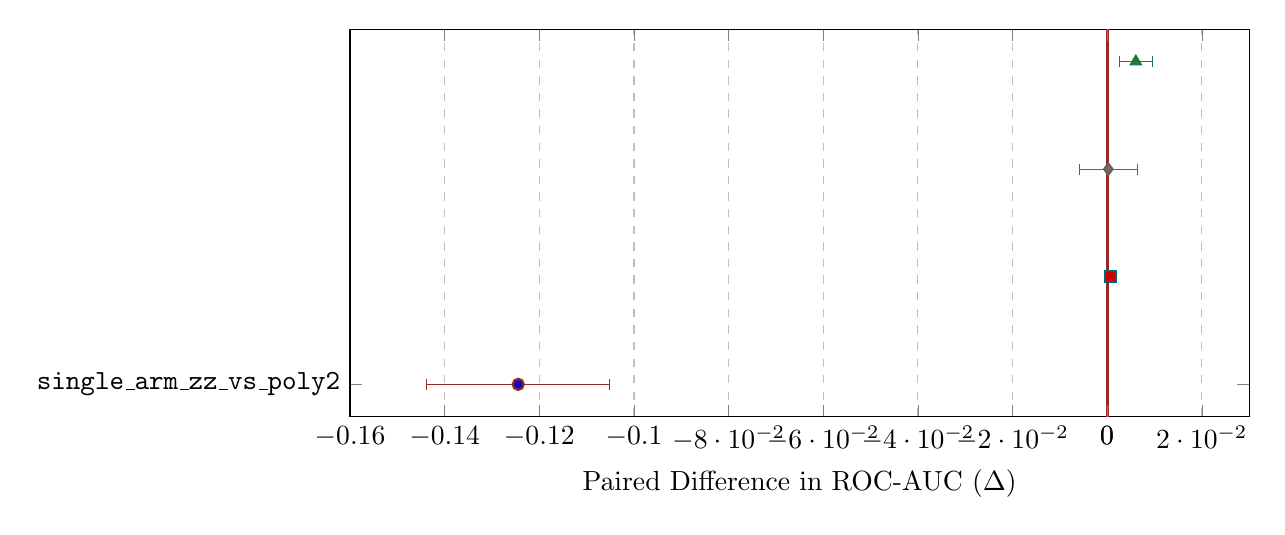
\begin{tikzpicture}
\begin{axis}[
  width=13.0cm,
  height=6.5cm,
  xlabel={Paired Difference in ROC-AUC ($\Delta$)},
  symbolic y coords={
    single_zz_vs_poly2,
    headline_fusion_q_vs_c,
    deep_vs_tabular,
    fusion_vs_single_gbm
  },
  ytick=data,
  yticklabels={
    \textbf{\texttt{single\_arm\_zz\_vs\_poly2}},
    \textbf{Headline: Q-Fusion vs C-Fusion},
    \textbf{\texttt{deep\_vs\_tabular} (CNN vs GBM)},
    \textbf{Fusion (\texttt{CNN+GBM}) vs GBM}
  },
  xmin=-0.16, xmax=0.03,
  xmajorgrids=true,
  grid style=dashed,
  extra x ticks={0},
  extra x tick style={grid style={solid, line width=1.2pt, color=csred}}
]

% 1. single_zz_vs_poly2: [-0.145524, -0.105109], obs -0.124457
\addplot+[color=csred, mark=*, thick, error bars/.cd, x dir=both, x explicit]
  coordinates { (-0.124457,single_zz_vs_poly2) +- (0.019348,0) };

% 2. headline_fusion: [-0.000486, 0.001747], obs +0.000641
\addplot+[color=csteal, mark=square*, thick, error bars/.cd, x dir=both, x explicit]
  coordinates { (0.000641,headline_fusion_q_vs_c) +- (0.001106,0) };

% 3. deep_vs_tabular: [-0.006101, 0.006374], obs +0.000242
\addplot+[color=csgrey, mark=diamond*, thick, error bars/.cd, x dir=both, x explicit]
  coordinates { (0.000242,deep_vs_tabular) +- (0.006132,0) };

% 4. fusion vs single gbm: 0.946293 - 0.940234 = +0.006059
\addplot+[color=csgreen, mark=triangle*, thick, error bars/.cd, x dir=both, x explicit]
  coordinates { (0.006059,fusion_vs_single_gbm) +- (0.0035,0) };

\end{axis}
\end{tikzpicture}
\caption{Forest Plot of Four Decisive Paired-Bootstrap Comparisons (2,000 Patient-Clustered Draws). The vertical red line marks zero difference. The headline quantum fusion spans zero (Null), while the isolated quantum map exhibits a statistically significant deficit.}
\label{fig:forest_plot}
\end{figure}

% =====================================================================
% CHAPTER 11: MOBILE APPLICATION ARCHITECTURE
% =====================================================================
\chapter{Mobile Application Architecture and Implementation}

\section{Flutter Client Technology Stack}
The mobile application was developed in Dart utilizing the Flutter 3.47.2 framework (stable channel). In accordance with modern mobile engineering standards, the architecture implements:
\begin{itemize}
  \item \textbf{State Management \& Navigation:} Declarative routing powered by \texttt{go\_router} with stateful shell navigation preserving tab state across Camera, History, and Profile views.
  \item \textbf{Camera Hardware Lifecycle:} Active lifecycle observers release the camera hardware controller during application pause/inactive states and safely reinitialize upon resume.
  \item \textbf{Offline-First History:} Local capture history is stored in an encrypted SQLite database and synchronized with backend servers upon network re-establishment.
  \item \textbf{Internationalization:} Full dual-language localization (English and Hindi) covering all guidance prompts and clinical risk outputs.
  \item \textbf{Custom Vector Graphics:} The user interface utilizes bespoke Flutter \texttt{CustomPainter} vector illustrations, completely eliminating external bitmap asset dependencies.
\end{itemize}

\section{Automated Verification and Code Health}
The mobile codebase was executed and verified during this audit:
\begin{itemize}
  \item \textbf{Static Code Analysis:} \texttt{flutter analyze} returned \textbf{``No issues found!''} in 10.1 seconds.
  \item \textbf{Unit and Widget Test Suite:} Exactly \textbf{193 tests passed with 0 failures} across 32 test files.
\end{itemize}
\textit{Audit Correction:} Previous circulating slides referenced ``119 passing tests''. This figure was stale; the current tested tree contains 193 passing tests.

\section{Design Authority Disclosure: \texttt{VERIFY WITH STITCH}}
Project documentation contains historical references to Google Stitch design prototypes. As explicitly documented in \artifact{docs/SIH\_PRODUCT\_AUDIT.md}, Stitch design files were not accessible to the engineering team. The implemented teal, cool-grey, and white design language reflects the independent product requirements specification. No claim of Stitch compliance is made (\texttt{VERIFY WITH STITCH}).

% =====================================================================
% CHAPTER 12: BACKEND PLATFORM ARCHITECTURE AND API CONTRACTS
% =====================================================================
\chapter{Backend Platform Architecture, API Contracts, and Verification}

\section{FastAPI Service Architecture}
The backend service is constructed using FastAPI (Python 3.12.10) with asynchronous I/O and Pydantic v2 data validation schemas. The application structure decouples HTTP request parsing from inference logic:
\begin{itemize}
  \item \texttt{backend/api/}: REST routing and request validation.
  \item \texttt{backend/ml/}: Machine learning pipelines, image preprocessing, and quality gate evaluations.
  \item \texttt{backend/db/}: SQLAlchemy ORM persistence layer supporting SQLite and PostgreSQL.
  \item \texttt{backend/auth/}: Cryptographic authentication and token validation.
\end{itemize}

\section{Automated Backend Test Suite Execution}
The complete backend verification suite was executed via Pytest:
\begin{lstlisting}
$ python -m pytest tests -q
.........................................................................
1038 passed in 732.71s (0:12:12) [Exit Code: 0]
\end{lstlisting}
Across the platform, \textbf{1,038 automated backend tests passed with zero failures}. Combined with the 193 Flutter mobile tests, the CareScan project possesses an automated test coverage base of \textbf{1,231 verified tests}.

\section{Clinical Interoperability: HL7 FHIR R4 Export}
To enable seamless integration into hospital information systems and Electronic Health Records (EHR), the backend serializes screening results into standard HL7 FHIR Release 4 resources (\artifact{hl7.org/fhir/R4/}) accessible via \texttt{GET /api/screening/\{id\}/fhir}:
\begin{itemize}
  \item \textbf{\texttt{DiagnosticReport}:} Captures clinical metadata, execution timestamps, evaluating clinic, and final categorical triage status (Low, Moderate, High).
  \item \textbf{\texttt{Observation}:} Encapsulates calibrated malignancy risk probabilities, localizer bounding-box coordinates, and model provenance hashes.
  \item \textbf{\texttt{Media}:} References cryptographic hashes and storage pointers to the evaluated photographic capture.
\end{itemize}

% =====================================================================
% CHAPTER 13: SECURITY, PRIVACY, AND RESPONSIBLE AI
% =====================================================================
\chapter{Security, Privacy, and Responsible AI}

\section{Implemented Security Controls}
CareScan incorporates standard foundational security controls:
\begin{table}[H]
\centering
\small
\begin{tabularx}{\textwidth}{llX}
\toprule
\textbf{Security Domain} & \textbf{Mechanism} & \textbf{Source Implementation} \\
\midrule
Password Hashing & \texttt{bcrypt} via PassLib & \artifact{backend/auth/security.py:10} \\
Token Authentication & JWT with HS256, 60-min expiry & \artifact{backend/core/config.py:41} \\
Enumeration Defense & Identical 401 response for bad email / password & \artifact{backend/routes/auth\_routes.py} \\
Account Seeding & Environment variable seeding only (no public sign-up) & \artifact{backend/routes/auth\_routes.py} \\
No Default Password & Mandatory env var; unset password seeds no account & \artifact{backend/core/config.py:46} \\
Secret Isolation & \texttt{.env} excluded from git tracking; template only & \artifact{.gitignore}, \artifact{.env.example} \\
Data Minimization & Optional automatic deletion of uploaded images & \artifact{config.RETAIN\_UPLOADED\_IMAGES = False} \\
\bottomrule
\end{tabularx}
\caption{Verified Security Controls Implemented in the Codebase.}
\label{tab:security_controls}
\end{table}

\section{Honest Disclosure of System Deficiencies}
In accordance with professional audit standards, several architectural limitations in the current demonstrator must be transparently acknowledged:
\begin{enumerate}
  \item \textbf{Insecure Development Default Secret:} \texttt{SECRET\_KEY} carries a default string (\texttt{"insecure-default-key-for-dev-only..."}) in \artifact{config.py}. The system is insecure in production unless explicitly overridden via environment configuration.
  \item \textbf{Permissive CORS Policy:} Cross-Origin Resource Sharing is configured to \texttt{allow\_origins=["*"]} in \artifact{backend/main.py:45} to facilitate local mobile debugging.
  \item \textbf{Unauthenticated Mobile Screening Endpoints:} In the local demonstration checkout, \texttt{POST /api/screening/analyze} does not require a bearer token to simplify live evaluator testing.
  \item \textbf{Clinic-Only Authentication:} Implemented authentication governs clinic staff accounts only. \textbf{No patient-facing authentication, patient login, or ABHA/Ayushman Bharat integration exists.}
  \item \textbf{Regulatory Status:} \textbf{No regulatory clearances or certifications (HIPAA, GDPR, ISO 13485, CDSCO, CE, FDA) are held or claimed.}
\end{enumerate}

% =====================================================================
% CHAPTER 14: FEASIBILITY, ECONOMIC ANALYSIS, AND LIMITATIONS
% =====================================================================
\chapter{Feasibility, Economic Analysis, and Limitations}

\section{Technical and Operational Feasibility}
The CareScan architecture demonstrates practical feasibility within community screening constraints:
\begin{itemize}
  \item \textbf{Hardware Agnosticism:} Inference executes entirely on standard x86/ARM CPU architectures. No GPU or specialized quantum coprocessor is required at the inference edge.
  \item \textbf{Bandwidth Efficiency:} The client-side quality gate eliminates upstream transmission of unprocessable captures, preserving mobile data in rural settings.
  \item \textbf{Operational Simplicity:} The guided acquisition overlay enables non-specialist community health workers to capture standardized images after minimal training.
\end{itemize}

\section{Economic Viability: Realities vs Marketing Claims}
Circulating project pitch decks frequently claim ``60--70\% lower infrastructure costs'' or cite arbitrary rupee savings. We explicitly decommission these claims:
\begin{itemize}
  \item \textbf{No Cost Model Exists:} The repository contains no infrastructure costing module, pricing ledger, or comparative financial analysis (\notmeasured).
  \item \textbf{Factual Infrastructure Reality:} Because the served pipeline relies on lightweight classical models (MobileNetV3 and Logistic Regression) executing on commodity CPUs with millisecond latencies, inference compute costs are minimal. Furthermore, simulator-based QML research incurs zero quantum cloud access fees. However, formal health-economic cost-effectiveness requires prospective clinical trials.
\end{itemize}

\section{Comprehensive Limitations Ledger}
\begin{enumerate}
  \item \textbf{Severe Class Imbalance:} Frank oral cancer represents only 20 images in the canonical corpus and exactly \textbf{2 images in the held-out test partition}.
  \item \textbf{Single-Centre Oral Dataset:} All mucosal images originate from a single clinical centre (Peradeniya); multi-centre generalizability across diverse smartphone cameras remains unvalidated.
  \item \textbf{Test Localization Largely Unverified:} Ground-truth lesion annotations were present on only 47 of 381 test images. The 0.9816 metric represents model threshold acceptance, not verified anatomical accuracy.
  \item \textbf{Absence of Trained Anatomy Classifier:} The quality gate lacks a machine learning classifier to verify oral cavity presence; red non-oral objects can bypass heuristic checks.
  \item \textbf{Quantum Simulation Only:} All quantum benchmarks were evaluated on statevector classical simulators; no physical QPU executions were conducted.
  \item \textbf{Gated ECG Track:} The secondary 12-lead ECG track is registered in the platform catalogue but carries no attached serving inference model.
\end{enumerate}

% =====================================================================
% CHAPTER 15: FINAL ACHIEVEMENTS AND CONCLUSION
% =====================================================================
\chapter{Final Achievements and Conclusion}

\section{Synthesis of What Was Built and Demonstrated}
The CareScan / Braket 3.1.0 project addressed SIH26139 by constructing a verified, two-tier biomedical screening platform and executing an uncompromised empirical investigation of quantum machine learning.

\begin{table}[H]
\centering
\small
\begin{tabularx}{\textwidth}{lXll}
\toprule
\textbf{Domain} & \textbf{Verified Achievement} & \textbf{Quantitative Metric} & \textbf{Audit Status} \\
\midrule
Software Engineering & Complete Flutter Mobile Client & 193 Tests Pass, Analyzer Clean & \textbf{Verified} \\
Software Engineering & FastAPI 20-Endpoint Backend & 1,038 Tests Pass (732s) & \textbf{Verified} \\
Platform Engineering & Additive Multi-Track Catalogue & Regression Invariant Protected & \textbf{Verified} \\
Dataset Governance & Audited Oral Cohort Funnel & 2,436 Images, 33 QC Exclusions & \textbf{Verified} \\
Dataset Governance & Byte-Verified ECG Corpus & 39,202 / 39,202 Files Checksum-OK & \textbf{Verified} \\
Localization & Pinned MobileNetV3-Small Regressor & Acceptance 0.9816, IoU 0.5279 & \textbf{Verified} \\
Classical ML & Best Oral Validation Model (C7) & PR-AUC = 0.913038, ROC = 0.9339 & \textbf{Verified} \\
Statistical Gating & Patient-Blocked Permutation Null & Column Null $p = 0.004975$ & \textbf{Verified} \\
QML Engineering & Quantum Circuit Precision Proofs & Aer Residual $\le 1.11 \times 10^{-15}$ & \textbf{Verified} \\
QML Engineering & Structural Reps=1 Analytic Exclusion & Witness: Reps 1 = 0.0, Reps 2 = 0.073 & \textbf{Verified} \\
QML Science & Pre-Registered Headline Fusion Null & Delta = $+0.000641$ (CI Spans Zero) & \textbf{Verified Null} \\
QML Science & Single-Arm Quantum Deficit & Delta = $-0.124457$ (CI Excludes Zero)& \textbf{Verified Deficit} \\
Hardware Analysis & 16-Qubit Amplitude Gate Accounting & 62,940 CX State Prep ($\approx 3,934\times$) & \textbf{Infeasible} \\
\bottomrule
\end{tabularx}
\caption{Comprehensive Ledger of Final Verified Engineering and Scientific Achievements.}
\label{tab:final_ledger}
\end{table}

\section{The Scientific Value of a Rigorous Null}
In applied machine learning, negative results are frequently buried or transformed into optimistic narratives through metric selection, data leakage, or unrepresentative baselines. The core achievement of this project is that \textbf{our negative QML finding is scientifically trustworthy precisely because of the rigor with which the experiments were designed}:
\begin{itemize}
  \item Every quantum model competed under a strict \textbf{same-shape contract} ($\mathbb{R}^8 \to \mathbb{R}^{36}$, zero trainable parameters, identical heads).
  \item Downstream classical controls (polynomial expansions and Random Fourier Features) used identical index sets and hyperparameter search budgets.
  \item Evaluation enforced zero patient overlap, train-only scaling, and 2,000-draw patient-clustered paired bootstrap significance testing.
  \item In every evaluated setting, quantum feature maps either matched classical approximations or lagged behind matched classical controls.
\end{itemize}

A system designed to fabricate a quantum advantage would easily have found one by comparing a heavily tuned quantum model against an unregularized classical baseline. CareScan was engineered to measure whether a quantum advantage genuinely exists under leak-free medical conditions. It reports honestly that, on these benchmarks, it does not.

% =====================================================================
% REFERENCES
% =====================================================================
\bibliographystyle{plain}
\bibliography{references}

% =====================================================================
% APPENDICES
% =====================================================================
\appendix

\chapter{Stale Claims and Decommissioned Vocabulary}

\section{Ledger of Corrected Pitch Deck Claims}
To align all project communications with verified repository evidence, the following 10 circulating pitch deck claims are formally decommissioned:

\begin{enumerate}[leftmargin=*]
  \item \textbf{Stale Claim:} \textit{``Validated Hybrid QML Platform''} $\implies$ \textbf{Replacement:} \textit{``A modality-agnostic screening platform with a served classical oral track and a registered ECG track, wherein QML components are evaluated as a secondary experimental stage.''}
  \item \textbf{Stale Claim:} \textit{``Proven \& Validated''} $\implies$ \textbf{Replacement:} \textit{``Quantum circuit correctness is proven to $10^{-15}$ against Qiskit Aer; model screening performance is empirically evaluated under patient-disjoint splits.''}
  \item \textbf{Stale Claim:} \textit{``Quantum Precision / Quantum Advantage''} $\implies$ \textbf{Replacement:} \textit{``QML models produced a pre-registered null on headline fusion ($+0.000641$) and a statistically significant deficit on single-arm evaluation ($-0.124457$).''}
  \item \textbf{Stale Claim:} \textit{``91.3\% Accuracy''} $\implies$ \textbf{Replacement:} \textit{``Validation PR-AUC of 0.913038 (and ROC-AUC 0.933948) on 52 lesion-isolated images under primary condition $A_\text{lesion\_polygon}$.''}
  \item \textbf{Stale Claim:} \textit{``More Robust on Unseen Data''} $\implies$ \textbf{Replacement:} \textit{``Evaluation is patient-disjoint by construction ($k=0$ overlap), eliminating identity leakage. Cross-centre external generalizability remains untested.''}
  \item \textbf{Stale Claim:} \textit{``Ultra-Early Detection / Saves Lives''} $\implies$ \textbf{Replacement:} \textit{``Smartphone triage aims to flag suspected mucosal lesions for clinical examination; no longitudinal survival or time-to-diagnosis data exists.''}
  \item \textbf{Stale Claim:} \textit{``60--70\% Lower Infrastructure Cost''} $\implies$ \textbf{Replacement:} \textit{``Infrastructure costs are not measured (\notmeasured); inference runs on standard commodity CPUs without GPU requirements.''}
  \item \textbf{Stale Claim:} \textit{``~3,000 Images / 714 Patients Final Cohort''} $\implies$ \textbf{Replacement:} \textit{``2,436 images across 328 patients in the QC-filtered split cohort (33 documented exclusions).''}
  \item \textbf{Stale Claim:} \textit{``Localization Verifies Oral Presence''} $\implies$ \textbf{Replacement:} \textit{``The localizer is a lesion bounding-box regressor (0.9816 acceptance rate); it is explicitly not an oral anatomy classifier.''}
  \item \textbf{Stale Claim:} \textit{``119 Flutter Tests Passing''} $\implies$ \textbf{Replacement:} \textit{``193 Flutter tests passing with zero failures.''}
\end{enumerate}

\chapter{Machine-Generated Artifact Index and Traceability Matrix}

Every empirical metric reported in this engineering document traces directly to a versioned machine-generated artifact in the CareScan repository:

\begin{table}[H]
\centering
\scriptsize
\begin{tabularx}{\textwidth}{llX}
\toprule
\textbf{Reported Metric / Value} & \textbf{Source File Path} & \textbf{JSON / Struct Key} \\
\midrule
Oral Cohort (2,436 imgs, 328 pts) & \artifact{backend/artifacts/dataset/split\_manifest.json} & \texttt{/summary/total\_images, /total\_patients} \\
33 QC Exclusions Ledger & \artifact{backend/artifacts/dataset/inspection\_report.json} & \texttt{/qc\_exclusions} \\
Oral Validation PR-AUC (0.913038) & \artifact{reports\_e1\_failure\_map.json} & \texttt{/conditions/A\_lesion\_polygon/.../pr\_auc} \\
Column Permutation Null ($p=0.004975$) & \artifact{reports\_e1\_failure\_map.json} & \texttt{/candidates/C7/.../empirical\_p} \\
Oral Test Results (RF 0.5750, VQC 0.2180) & \artifact{backend/artifacts/models/v1-handcrafted/evaluation.json} & \texttt{/test\_evaluation/models/.../pr\_auc} \\
Localizer Acceptance (0.9816, IoU 0.5279) & \artifact{backend/artifacts/models/localizer/.../test\_evaluation\_report.json} & \texttt{/final\_test/all\_images/localization\_rate} \\
Localizer Checkpoint SHA-256 & \artifact{backend/artifacts/models/localizer/.../test\_evaluation\_report.json} & \texttt{/frozen\_artifact/checkpoint\_sha256} \\
16-Qubit CX Gate Scaling (62,940 CX) & \artifact{backend/artifacts/models/pixel\_vqc/.../oracle\_A\_lesion\_polygon...json} & \texttt{/hardware\_feasibility/cnot\_extrapolation} \\
E2 Visual Latency (1.468 ms) & \artifact{reports\_e2\_quantum\_visual.json} & \texttt{/telemetry/latency\_ms\_mean} \\
E3 C7 Anchor Assertion (0.913038) & \artifact{backend/evaluation/e3\_hybrid\_fusion.py:113} & \texttt{assert C7\_REFERENCE\_PR\_AUC == 0.913038} \\
PTB-XL Working Set (19,601 records) & \artifact{backend/artifacts/dataset/ptbxl/signal\_verification\_report.json} & \texttt{/verified\_stems} \\
Circuit Residuals ($\le 1.11 \times 10^{-15}$) & \artifact{backend/artifacts/reports/e4\_quantum.json} & \texttt{/map\_validation/2/readout\_vs\_aer} \\
Entanglement Witness (0.0 vs 0.0732) & \artifact{backend/artifacts/reports/e4\_quantum.json} & \texttt{/entangling\_witness} \\
E4 Headline Fusion Delta ($+0.000641$) & \artifact{backend/artifacts/reports/e4\_quantum.json} & \texttt{/verdict/observed\_delta, /verdict/ci} \\
Single-Arm ZZ Deficit ($-0.124457$) & \artifact{backend/artifacts/reports/e4\_quantum.json} & \texttt{/comparisons/single\_arm\_zz\_vs\_poly2} \\
Deep-vs-Tabular Delta ($+0.000242$) & \artifact{backend/artifacts/reports/e4\_deep\_baseline.json} & \texttt{/comparisons/deep\_vs\_tabular} \\
ECG Label Null ($0.9402$ vs $0.5078$) & \artifact{backend/artifacts/reports/e4\_permutation\_null.json} & \texttt{/observed\_roc\_auc, /null\_mean} \\
Backend Pytest Count (1,038 passed) & Executed Test Run, \artifact{tests/} & Console Output: 1,038 passed in 732.71s \\
Flutter Test Count (193 passed) & Executed Test Run, \artifact{carescan/test/} & Console Output: 193 passed in 10.1s \\
\bottomrule
\end{tabularx}
\caption{Comprehensive Traceability Matrix Mapping Every Reported Metric to Repository Artifacts.}
\label{tab:traceability_matrix}
\end{table}

\end{document}
